\documentclass[12pt, letterpaper]{article}
%\documentclass[12pt, letterpaper, titlepage]{article}

\usepackage{amsmath}
\usepackage{booktabs}
\usepackage{amsthm}
\usepackage{graphicx}
\usepackage[margin=1in]{geometry}
\usepackage{hyperref}
\hypersetup{colorlinks = true, linkcolor = blue, citecolor=blue, urlcolor = blue}
\usepackage{natbib}
\usepackage{enumitem}
\usepackage{setspace}

\usepackage[]{lineno}
\linenumbers*[1]
% %% patches to make lineno work better with amsmath
\newcommand*\patchAmsMathEnvironmentForLineno[1]{%
 \expandafter\let\csname old#1\expandafter\endcsname\csname #1\endcsname
 \expandafter\let\csname oldend#1\expandafter\endcsname\csname end#1\endcsname
 \renewenvironment{#1}%
 {\linenomath\csname old#1\endcsname}%
 {\csname oldend#1\endcsname\endlinenomath}}%
\newcommand*\patchBothAmsMathEnvironmentsForLineno[1]{%
 \patchAmsMathEnvironmentForLineno{#1}%
 \patchAmsMathEnvironmentForLineno{#1*}}%

\AtBeginDocument{%
 \patchBothAmsMathEnvironmentsForLineno{equation}%
 \patchBothAmsMathEnvironmentsForLineno{align}%
 \patchBothAmsMathEnvironmentsForLineno{flalign}%
 \patchBothAmsMathEnvironmentsForLineno{alignat}%
 \patchBothAmsMathEnvironmentsForLineno{gather}%
 \patchBothAmsMathEnvironmentsForLineno{multline}%
}

% control floats
\renewcommand\floatpagefraction{.9}
\renewcommand\topfraction{.9}
\renewcommand\bottomfraction{.9}
\renewcommand\textfraction{.1}
\setcounter{totalnumber}{50}
\setcounter{topnumber}{50}
\setcounter{bottomnumber}{50}

\newcommand{\jy}[1]{\textcolor{blue}{JY: #1}}
\newcommand{\eds}[1]{\textcolor{red}{EDS: (#1)}}

% NOTE: To produce blinded version, replace "0" with "1" below.
\newcommand{\blind}{0}


%\title{On Misuses of the Kolmogorov--Smirnov Test for One-Sample Goodness-of-Fit}
%
%\author{Anthony Zeimbekakis\\
%%   \href{mailto:anthony.zeimbekakis@uconn.edu}
%% {\nolinkurl{anthony.zeimbekakis@uconn.edu}}\\
  %Elizabeth D.  Schifano\\
  %Jun Yan\\[1ex]
  %Department of Statistics, University of Connecticut\\
%}
%\date{}

\begin{document}
%\maketitle

\if0\blind
{
  \title{\bf Paper about Something}
  \author{Mathew Chandy\\[1ex]
%   \href{mailto:mathew.chandy@uconn.edu}
% {\nolinkurl{mathew.chandy@uconn.edu}}\\
  Department of Statistics, University of Connecticut\\
}
\date{}
  \maketitle
} \fi

\if1\blind
{
  \bigskip
  \bigskip
  \bigskip
  \begin{center}
    {\LARGE\bf Paper about Something}
\end{center}
  \bigskip
} \fi


\doublespace

\begin{abstract}
Lorem ipsum dolor sit amet, consectetur adipiscing elit, sed do eiusmod tempor 
incididunt ut labore et dolore magna aliqua. Bibendum enim facilisis gravida 
neque convallis a cras semper auctor. Mauris pharetra et ultrices neque ornare 
aenean. Cursus risus at ultrices mi tempus imperdiet nulla malesuada. Sed arcu 
non odio euismod lacinia at quis risus sed. Id aliquet lectus proin nibh nisl 
condimentum. At in tellus integer feugiat. Gravida cum sociis natoque penatibus 
et magnis dis parturient. Aliquet risus feugiat in ante metus. Sed turpis 
tincidunt id aliquet. Semper quis lectus nulla at volutpat. Tincidunt arcu non 
sodales neque sodales ut etiam sit. Quis risus sed vulputate odio ut. Ac turpis 
egestas maecenas pharetra convallis posuere morbi.

\bigskip
\noindent{\sc Keywords}:
statistics;
data science.
\end{abstract}

%\doublespace

\section{Introduction}
\label{sec:intro}

Lorem ipsum dolor sit amet, consectetur adipiscing elit, sed do eiusmod tempor 
incididunt ut labore et dolore magna aliqua. Sollicitudin aliquam ultrices 
sagittis orci a scelerisque purus semper eget. Adipiscing bibendum est ultricies 
integer quis auctor elit sed vulputate. Egestas dui id ornare arcu odio ut. 
Dictum at tempor commodo ullamcorper a lacus vestibulum sed. Vel pharetra vel 
turpis nunc eget lorem dolor sed. Condimentum vitae sapien pellentesque habitant 
morbi tristique senectus. An example of a math expression is 
$3x^2 + 2(b + \lambda)$. A condimentum vitae 
sapien pellentesque habitant morbi 
tristique senectus. Dolor sit amet consectetur adipiscing elit. Tristique nulla 
aliquet enim tortor. Purus viverra accumsan in nisl. Quam lacus suspendisse 
faucibus interdum posuere lorem ipsum. Tincidunt praesent semper feugiat nibh 
sed. Amet porttitor eget dolor morbi non arcu risus quis. Morbi tristique 
senectus et netus et malesuada fames ac turpis. Iaculis eu non diam phasellus 
vestibulum lorem sed. Dolor sit amet consectetur adipiscing elit duis tristique.

Urna neque viverra justo nec. Justo donec enim diam vulputate ut pharetra. Vitae 
tortor condimentum lacinia quis vel eros. Molestie nunc non blandit massa. 
Rutrum quisque non tellus orci ac auctor augue. \citet{westgate2013travel} is a
good example of a paper. Sem viverra aliquet 
eget sit amet tellus cras adipiscing enim. Egestas tellus rutrum tellus 
pellentesque eu tincidunt tortor. Eget nulla facilisi etiam dignissim diam quis 
enim. Ut sem viverra aliquet eget sit. Interdum velit euismod in pellentesque 
massa. Luctus accumsan tortor posuere ac ut. Urna id volutpat lacus laoreet non 
curabitur gravida arcu ac. Sed ullamcorper morbi tincidunt ornare massa eget.

Quis lectus nulla at volutpat diam. Vulputate ut pharetra sit amet aliquam id 
diam maecenas. Eget velit aliquet sagittis id consectetur purus ut. Blandit 
aliquam etiam erat velit. Gravida rutrum quisque non tellus orci ac auctor augue 
mauris. Senectus et netus et malesuada fames ac turpis egestas. Velit euismod in 
pellentesque massa placerat duis ultricies lacus sed. Congue nisi vitae suscipit 
tellus mauris a diam maecenas sed. Turpis egestas maecenas pharetra convallis 
posuere. There many other examples of interesting papers 
\citep{alfons2013sparse}. Vel elit 
scelerisque mauris pellentesque pulvinar pellentesque. In 
massa tempor nec feugiat nisl pretium fusce id. Amet commodo nulla facilisi 
nullam vehicula ipsum a arcu cursus. Amet consectetur adipiscing elit duis 
tristique. Nisl nunc mi ipsum faucibus vitae. Eu mi bibendum neque egestas 
congue. Dui faucibus in ornare quam. Sed odio morbi quis commodo. Id aliquet 
risus feugiat in ante metus dictum at. Mattis aliquam faucibus purus in.

The remainder of the paper is organized in the following manner:
Section~\ref{sec:methods} outlines the methods used in this study, 
Section~\ref{sec:results} discusses the results, 
and Section~\ref{sec:conclusion} goes over the significance, limitations, and
some topics to investigate in the future. Finally, we conclude with an appendix
on something.


\section{Methods}
\label{sec:methods}

Mi tempus imperdiet nulla malesuada pellentesque elit eget. Libero enim sed 
faucibus turpis in eu mi bibendum neque. Ipsum a arcu cursus vitae congue mauris 
rhoncus. Neque viverra justo nec ultrices dui sapien eget. Elit ut aliquam purus 
sit amet luctus venenatis. Habitant morbi tristique senectus et netus et. Nullam 
non nisi est sit. Consectetur adipiscing elit duis tristique sollicitudin nibh 
sit amet commodo. Sociis natoque penatibus et magnis dis parturient montes 
nascetur ridiculus. Duis ut diam quam nulla porttitor. 
\begin{equation}
\label{eq:normcdf}
{\displaystyle F(x) = \Phi ({\frac {x-\mu }{\sigma }})={\frac {1}{2}}\left[1+\operatorname {erf} \left({\frac {x-\mu }{\sigma {\sqrt {2}}}}\right)\right]}
\end{equation}

Ac tortor dignissim 
convallis aenean et tortor. Augue interdum velit euismod in pellentesque massa 
placerat duis ultricies. Equation~\ref{eq:massenergy} was made famous by Albert
Einstein. Duis at consectetur lorem donec massa sapien faucibus 
et molestie. Lectus proin nibh nisl condimentum id venenatis a condimentum. 
Urna porttitor rhoncus dolor purus non. 
\begin{equation}
\label{eq:massenergy}
E=MC^2
\end{equation}

Sit amet justo donec enim diam 
vulputate. Pretium quam vulputate dignissim suspendisse in. Massa sapien 
faucibus et molestie. Sollicitudin tempor id eu nisl nunc mi ipsum faucibus. 
Tempus iaculis urna id volutpat lacus.


Tincidunt vitae semper quis lectus nulla at volutpat diam. Eget egestas purus 
viverra accumsan. Sit amet cursus sit amet. Risus viverra adipiscing at in 
tellus integer. Pharetra vel turpis nunc eget lorem dolor sed viverra ipsum. 
Accumsan in nisl nisi scelerisque eu. Maecenas pharetra convallis posuere morbi 
leo urna molestie at elementum. The CDF for a normal distribution is displayed 
in Equation~\ref{eq:normcdf}. Aliquam purus sit amet luctus venenatis lectus. 
Nulla facilisi cras fermentum odio eu feugiat pretium. Non odio euismod lacinia 
at quis risus sed vulputate odio. Massa tempor nec feugiat nisl pretium fusce id 
velit ut. Sapien pellentesque habitant morbi tristique senectus et. Vel turpis 
nunc eget lorem dolor sed viverra. Purus semper eget duis at tellus at urna 
condimentum mattis. Ornare aenean euismod elementum nisi quis eleifend. Gravida 
quis blandit turpis cursus in hac habitasse platea.

\section{Results}
\label{sec:results}

Tincidunt vitae semper quis lectus nulla at volutpat diam. Eget egestas purus 
viverra accumsan. Sit amet cursus sit amet. Risus viverra adipiscing at in 
tellus integer. Pharetra vel turpis nunc eget lorem dolor sed viverra ipsum. 
Accumsan in nisl nisi scelerisque eu. Maecenas pharetra convallis posuere morbi 
leo urna molestie at elementum. Aliquam purus sit amet luctus venenatis lectus. 
Nulla facilisi cras fermentum odio eu feugiat pretium. Non odio euismod lacinia 
at quis risus sed vulputate odio. Massa tempor nec feugiat nisl pretium fusce id 
velit ut. Sapien pellentesque habitant morbi tristique senectus et. Vel turpis 
nunc eget lorem dolor sed viverra. Purus semper eget duis at tellus at urna 
condimentum mattis. Ornare aenean euismod elementum nisi quis eleifend. Gravida 
quis blandit turpis cursus in hac habitasse platea.

\begin{center}
\label{tab:cooltable}
\begin{tabular}{||c c c c||} 
 \hline
 Col1 & Col2 & Col2 & Col3 \\ [0.5ex] 
 \hline\hline
 1 & 2 & 1 & 2 \\ 
 \hline
 2 & 4 & 4 & 4 \\
 \hline
 3 & 6 & 9 & 8 \\
 \hline
 4 & 8 & 16 & 16 \\
 \hline
 5 & 10 & 25 & 32 \\ [1ex] 
 \hline
\end{tabular}
\end{center}

\begin{figure}[t]
\label{fig:coolfig}
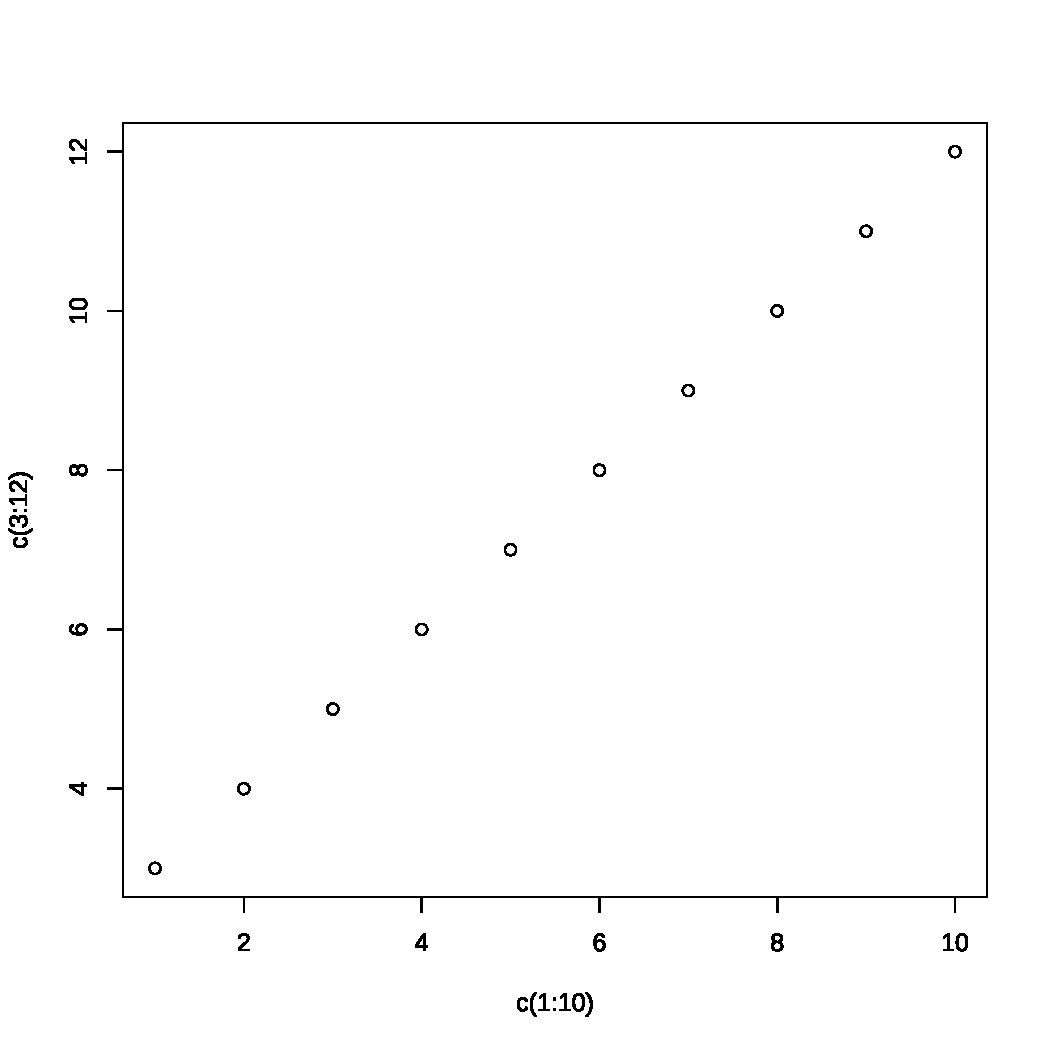
\includegraphics[width=8cm]{fig}
\centering
\end{figure}

Table~\ref{tab:cooltable} displays some interesting information. 
Lorem ipsum dolor sit amet, consectetur adipiscing elit, sed do eiusmod tempor 
incididunt ut labore et dolore magna aliqua. Sollicitudin aliquam ultrices 
sagittis orci a scelerisque purus semper eget. Adipiscing bibendum est ultricies 
integer quis auctor elit sed vulputate. Egestas dui id ornare arcu odio ut. 
Dictum at tempor commodo ullamcorper a lacus vestibulum sed. Vel pharetra vel 
turpis nunc eget lorem dolor sed. Condimentum vitae sapien pellentesque habitant 
morbi tristique senectus. A condimentum vitae sapien pellentesque habitant morbi 
tristique senectus. Dolor sit amet consectetur adipiscing elit. Tristique nulla 
aliquet enim tortor. Purus viverra accumsan in nisl. Quam lacus suspendisse 
faucibus interdum posuere lorem ipsum. Tincidunt praesent semper feugiat nibh 
sed. Amet porttitor eget dolor morbi non arcu risus quis. Morbi tristique 
senectus et netus et malesuada fames ac turpis. Iaculis eu non diam phasellus 
vestibulum lorem sed. Dolor sit amet consectetur adipiscing elit duis tristique.
Figure~\ref{fig:coolfig} also exhibits something informative.

\section{Conclusion}
\label{sec:conclusion}

Dictum at tempor commodo ullamcorper a lacus vestibulum sed. Vel pharetra vel 
turpis nunc eget lorem dolor sed. Condimentum vitae sapien pellentesque habitant 
morbi tristique senectus. A condimentum vitae sapien pellentesque habitant morbi 
tristique senectus. Here is another math expression: $\Sigma x(\phi + 3)$. Dolor 
sit amet consectetur adipiscing elit. Tristique nulla 
aliquet enim tortor. Purus viverra accumsan in nisl. Quam lacus suspendisse 
faucibus interdum posuere lorem ipsum. Tincidunt praesent semper feugiat nibh 
sed. 

\appendix

\section{Appendix: Nonparametric Bootstrap for KS Test with Fitted Parameters}



\bibliographystyle{asa}
\bibliography{citations}


\end{document}

